\documentclass[border=3pt]{standalone}
% Shared preamble for standalone figures (same fonts/colours as the paper).
\usepackage[T1]{fontenc}
\usepackage{lmodern}
\usepackage{amsmath,amssymb}
\usepackage[dvipsnames,svgnames]{xcolor}
\usepackage{tikz}
\usetikzlibrary{arrows.meta,positioning,calc,shapes.geometric,decorations.pathreplacing,shadings}
\usepackage{pgfplots}
\pgfplotsset{compat=1.18}
\usepgfplotslibrary{fillbetween}
\definecolor{pgrey}{HTML}{EEEEEE}
\definecolor{ppink}{HTML}{F8D7DA}
\definecolor{ppeach}{HTML}{FDE5C8}
\definecolor{porange}{HTML}{FBC78D}
\definecolor{pgreen}{HTML}{D4F7D4}
\definecolor{ppurple}{HTML}{EFE3F7}
\definecolor{pblue}{HTML}{DCE8F7}
\definecolor{dgreen}{HTML}{2E8B2E}
\definecolor{dpink}{HTML}{C2185B}
\definecolor{dorange}{HTML}{E07B00}
\definecolor{dblue}{HTML}{1F4E9E}
\definecolor{dpurple}{HTML}{7B3FA0}
\definecolor{gold}{HTML}{E0A800}
\tikzset{
  blk/.style={draw=black!70,rounded corners=2pt,minimum height=0.8cm,minimum width=1.9cm,
              align=center,font=\sffamily\footnotesize,inner sep=3pt},
  arr/.style={-{Stealth[length=2.2mm]},thick,black!75},
  darr/.style={-{Stealth[length=2mm]},dashed,thick},
  lbl/.style={font=\itshape\scriptsize},
}

\begin{document}
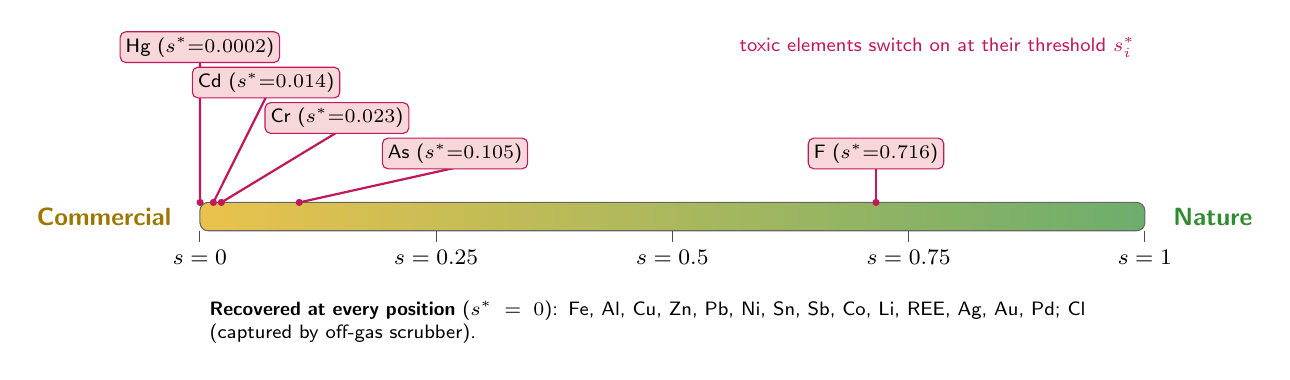
\begin{tikzpicture}[x=12cm,y=1cm]
\shade[left color=gold!70,right color=dgreen!70,rounded corners=3pt] (0,-0.18) rectangle (1,0.18);
\draw[black!60,rounded corners=3pt] (0,-0.18) rectangle (1,0.18);
\foreach \x/\t in {0/0,0.25/0.25,0.5/0.5,0.75/0.75,1/1}{
  \draw[black!70] (\x,-0.18) -- (\x,-0.32);
  \node[font=\footnotesize,below] at (\x,-0.3) {$s=\t$};}
\node[font=\sffamily\small\bfseries,text=gold!70!black,anchor=east] at (-0.02,0) {Commercial};
\node[font=\sffamily\small\bfseries,text=dgreen,anchor=west] at (1.02,0) {Nature};
% activation thresholds (labels in one row, leader lines to each threshold)
\foreach \s/\el/\lx/\ly/\val in {0.000196/Hg/0.0/1.95/0.0002,0.01426/Cd/0.07/1.5/0.014,0.02266/Cr/0.145/1.05/0.023,0.1051/As/0.27/0.6/0.105,0.7155/F/0.7155/0.6/0.716}{
  \draw[dpink,thick] (\s,0.18) -- (\lx,\ly+0.02);
  \fill[dpink] (\s,0.18) circle (1.3pt);
  \node[draw=dpink,fill=ppink,rounded corners=2pt,font=\sffamily\scriptsize,inner sep=2pt,anchor=south] at (\lx,\ly) {\el\ ($s^\ast{=}\val$)};}
\node[font=\sffamily\scriptsize,align=left,anchor=north west,text width=11.6cm] at (0,-0.95)
 {\textbf{Recovered at every position} ($s^\ast=0$): Fe, Al, Cu, Zn, Pb, Ni, Sn, Sb, Co, Li, REE, Ag, Au, Pd; Cl (captured by off-gas scrubber).};
\node[font=\sffamily\scriptsize,text=dpink,anchor=south east] at (1,1.9) {toxic elements switch on at their threshold $s^\ast_i$};
\end{tikzpicture}
\end{document}
